% ****** Start of file apssamp.tex ******
%
%   This file is part of the APS files in the REVTeX 4.2 distribution.
%   Version 4.2a of REVTeX, December 2014
%
%   Copyright (c) 2014 The American Physical Society.
%
%   See the REVTeX 4 README file for restrictions and more information.
%
% TeX'ing this file requires that you have AMS-LaTeX 2.0 installed
% as well as the rest of the prerequisites for REVTeX 4.2
%
% See the REVTeX 4 README file
% It also requires running BibTeX. The commands are as follows:
%
%  1)  latex apssamp.tex
%  2)  bibtex apssamp
%  3)  latex apssamp.tex
%  4)  latex apssamp.tex
%
\documentclass[%
 reprint,
%superscriptaddress,
%groupedaddress,
%unsortedaddress,
%runinaddress,
%frontmatterverbose, 
%preprint,
%preprintnumbers,
%nofootinbib,
%nobibnotes,
%bibnotes,
 amsmath,amssymb,
 aps,
%pra,
%prb,
%rmp,
%prstab,
%prstper,
%floatfix,
]{revtex4-2}

\usepackage{graphicx}% Include figure files
\usepackage{dcolumn}% Align table columns on decimal point
\usepackage{bm}% bold math
\usepackage{glossaries}
\usepackage{hyperref}% add hypertext capabilities
\usepackage{diagbox}

%\usepackage[mathlines]{lineno}% Enable numbering of text and display math
%\linenumbers\relax % Commence numbering lines

%\usepackage[showframe,%Uncomment any one of the following lines to test 
%%scale=0.7, marginratio={1:1, 2:3}, ignoreall,% default settings
%%text={7in,10in},centering,
%%margin=1.5in,
%%total={6.5in,8.75in}, top=1.2in, left=0.9in, includefoot,
%%height=10in,a5paper,hmargin={3cm,0.8in},
%]{geometry}
\makeglossaries  % This command prepares the package to process glossary entries.
\loadglsentries{glossary.tex}
\begin{document}

\preprint{APS/123-QED}

\title{G21cmFit: A Python Package For Parameter Estimation of Global 21cm Signal}
%\thanks{A footnote to the article title}%

\author{Aryana Haghjoo$^{1,2}$}
\email{aryana.haghjoo@mail.mcgill.ca}
 %\altaffiliation[Also at ]{Physics Department, XYZ University.}
\author{Jonathan Sievers$^{1,2}$}%
\author{Oscar Hernandez$^{1,3}$}
\affiliation{%
$^1$Department of Physics, McGill University, 3600 Rue University, Montréal, QC H3A 2T8, Canada\\
$^2$Trottier Space Institute, 3550 Rue University, Montréal, QC H3A 2A7, Canada\\
$^3$Marianopolis College, 4873 Westmount Ave., Westmount, QC H3Y 1X9, Canada
}%

\date{\today}% It is always \today, today,
             %  but any date may be explicitly specified

\begin{abstract} 
Constraining the period between the dark ages and reionization has recently emerged as one of the challenges of modern radio astronomy. The motivation behind this interest is the fact that there is a clear correlation between the key features of the global $21cm$ signal and underlying astrophysical properties of the high redshift Universe. These correlations can be used to directly link measurements of the global $21cm$ signal to astrophysical quantities. Moreover, the global $21cm$ signal is a novel probe of physics beyond the standard model of cosmology and astrophysics, and the majority of these proposed non-standard mechanisms are expected to leave their footprints on the value of physical parameters. Therefore, the urge to perform proper parameter estimation on the corresponding observational data is undeniable. In this work, we introduce \emph{G21cmFit}, an efficient Python package to estimate the astrophysical parameters of the global 21cm signal. This package takes advantage of \gls{mcmc} combined with the \gls{lm} algorithm to fit theoretical models to mock/experimental data of global $21cm$ signal. Conducting such studies will result in a better understanding of the physics governing the dark ages and cosmic dawn.
\end{abstract}

\keywords{Parameter Estimation, Global 21cm Signal}
                              %display desired
\maketitle

%\tableofcontents

\section{Background and Introduction}
The global $21cm$ signal is the average over the brightness temperature of the $21cm$ line across the entire sky. It is a measure of the overall state of the \gls{igm} and presents itself as an excess absorption or emission in different redshift regions. This radiation is a piece of observational evidence for certain characteristics of the \gls{igm} in the early universe (e.g., temperature, density, and reionization state). These properties are determined by the complex interplay between the cosmic radiation field, the formation and evolution of the first stars and galaxies, and the feedback processes that these sources exert on their surroundings\cite{21century}.\par

Three competing processes influence the spin temperature of $21cm$ signal: 1) interaction of $21cm$ photons with the radio background (mostly \gls{cmb}), 2) collisions with other particles (a mixture of hydrogen atoms, free electrons, and protons with hydrogen atoms as the leading component), and 3) resonant scattering of \gls{lya} photons that cause a spin-flip transition with through the meddling of an intermediate excited state. Therefore, the spin temperature is expressed using the equilibrium between these mechanisms and their corresponding coefficients \cite{low_frequency,21century}:
\begin{equation}
    T^{-1}_S = \frac{T^{-1}_\gamma + x_\alpha T^{-1}_\alpha + x_c T^{-1}_K}{1 + x_\alpha + x_c},
\end{equation}
Where $T_\gamma$ is the temperature of the surrounding bath of radio photons ($T_\gamma = T_{CMB}$). $T_\alpha$ is the color temperature of the \gls{lya} radiation field (at the \gls{lya} frequency), and $T_K$ is the kinetic temperature of gas. $x_c$ and $x_\alpha$ are the coupling coefficients due to atomic collisions and scattering of \gls{lya} photons, respectively. The spin temperature becomes strongly coupled to the gas temperature when the terms with coupling coefficients become dominant: $x_c + x_\alpha \gtrsim 1$. On the other hand, it relaxes to $T_\gamma$ when the coefficients are relatively small: $x_c + x_\alpha << 1$ \cite{21century, low_frequency}. \par
Averaging over the values of disparity between the $21cm$ line and the \gls{cmb} temperature, provides the differential brightness temperature of global $21cm$ signal \cite{low_frequency}:
\begin{equation}
    \delta T_b \approx 27 \left(1- \bar{x}_i\right) \left(\frac{\Omega_{b, 0}h^2}{0.023}\right) \left( \frac{0.15}{\Omega_{m, 0}h^2} \frac{1+z}{10}\right)^{1/2}\left(1-\frac{T_\gamma}{T_S}\right)
    \label{eq:global_curve}
\end{equation}
Where $x_i$ is the ionization fraction, and $h$ is the dimensionless Hubble constant. $\Omega_{b, 0}$ and $\Omega_{m, 0}$ are the ratio of the current energy density of baryonic and total matter with respect to the critical energy density of the universe. Figure \ref{fig:global_signal_pritchard_loeb} shows the evolution of the above equitation in the cosmic history.\par
The importance of parameter estimation for the global 21cm signal lies in its potential to provide crucial insights into the astrophysical properties of the high redshift Universe. This interest stems from the strong correlation observed between key features of the global 21cm signal and underlying astrophysical characteristics. By establishing these correlations, it becomes possible to directly connect measurements of the global 21cm signal to various astrophysical quantities.
Furthermore, the global 21cm signal serves as a valuable tool for exploring physics beyond the standard model of cosmology and astrophysics. Various proposed non-standard mechanisms are expected to leave distinct imprints on the physical parameters, and the global 21cm signal can act as a novel probe to detect such effects. Consequently, there is a compelling need to conduct proper parameter estimation on the observational data related to the global 21cm signal to understand and interpret its implications accurately. Therefore, we dedicate this study to the construction of a firm computational framework specifically designed for the global 21cm parameter estimation.\par
Besides all the above-mentioned applications, the global $21cm$ signal is a \textbf{strong probe for non-standard physics} during the dark ages and \gls{eor}. It has the potential to shed light on mysteries surrounding dark matter/dark energy, the existence of cosmic strings, and even certain particle interaction  \cite{dark_nature_21, constrain_dm_21, cosmic_string_brandenberger, ee_interaction_21, neutrino_21}. This capacity of the global $21cm$ signal is the main motivation of this research.
In this paper, we introduce \emph{G21cmFit}, which is a Python package designed to estimate the astrophysical parameters of the global $21cm$ signal. Previous studies have examined various computational algorithms to accomplish this task. The efforts include \gls{mcmc} \cite{pe_mcmc_1, pe_mcmc_2}, \gls{ann} \cite{pe_nn_1}, and even Fisher Matrix approaches \cite{pe_fisher_2}. This package employs both \gls{lm} and \gls{mcmc} fitting algorithms. The theoretical curve is generated using \gls{ares}, which is a Python package specifically designed for simulating the global $21cm$ signal curves.\par
In section \ref{sec:method} we thoroughly discuss the employed fitting method and its characteristics. Section \ref{sec:package} introduces the package and its dependencies. In section \ref{sec:evaluation}, we perform analysis using a mock data set to evaluate the performance of the algorithm.\par
\begin{figure}[h!]

\centering
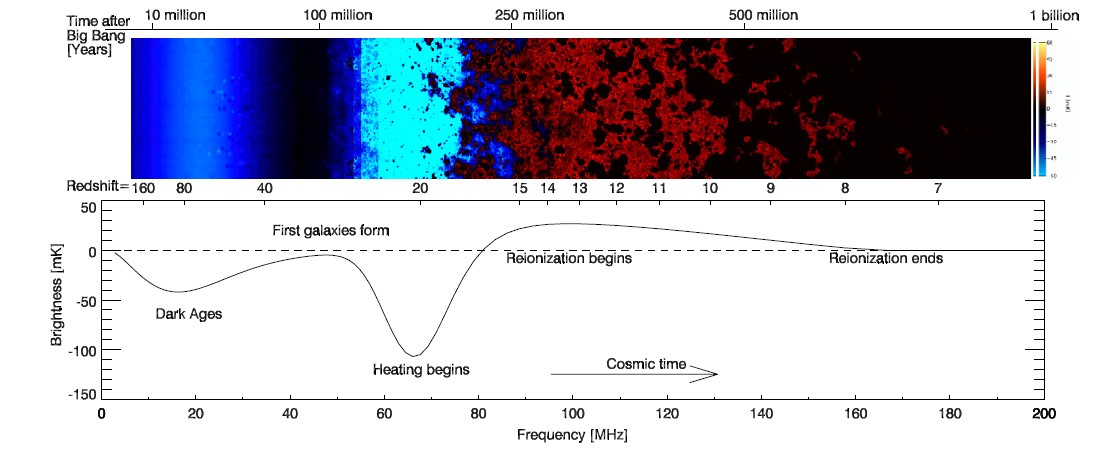
\includegraphics[scale =0.45]{global_signal_pritchard_loeb.jpg}
\caption[Time evolution of the fluctuations in the $21cm$ differential brightness temperature]{Time evolution of the fluctuations in the $21cm$ differential brightness temperature (solid line). The top panel is a color plot demonstrating fluctuations arising from variations in density. The coloration clearly depicts the two absorption phases of $21cm$ brightness temperature (coupling of $T_S$ to $T_K$, blue regions), emission phase (red regions), and the interval where it disappears completely (coupling of $T_S$ to $T_\gamma$, black region). The lower panel represents the evolution of sky-average (global) $21cm$ signal from the dark ages to the reionization. The frequency range of the absorption and emission regions exactly matches the corresponding regions in the upper panel. The precise details of the shape of this signal are still unidentified due to our lack of knowledge on the nature of early sources\cite{liu2013global}. Figure from Pritchard and Loeb, 2011 \cite{21century}.}
\label{fig:global_signal_pritchard_loeb}
\end{figure}
%------------------------------------------------------------------------------------------------------------
\section{Methodology}
\label{sec:method}
insights from the gradient, drawing samples (generating correlated noise with Eigenvalue decomposition)\\
 Sampling algorithms such as \gls{mcmc} are capable of exploring the entire likelihood surface in situations where it is feasible. On the other hand, neural networks are typically employed for problems where comprehensive mapping of the entire likelihood surface becomes excessively complex. This distinction positions \gls{mcmc} as advantageous for global 21cm applications.\par
We proceed by introducing the main parameter estimation algorithm used in our study, which is a combination of \gls{lm} and \gls{mcmc}. We explain the reason behind utilizing both of these algorithms for this particular fitting challenge and provide a detailed explanation of the procedure to combine them.\par
\gls{mcmc} is a computationally heavy algorithm due to its iterative nature. If the chi-square calculation process on each step is also a time-consuming task, the \gls{mcmc} will experience a rather long run-time before reaching the converged state. One of the proposed methods to deal with this issue and help the \gls{mcmc} to converge faster is to use the insights provided by the outputs of \gls{lm}\footnote{It is worth mentioning again that our sole rationale to use \gls{lm} in our application is to generate a covariance matrix for the MCMC.}.\par
We previously discussed that the parameters of a model might be correlated with each other, and the strength of this correlation is dictated by the elements of the covariance matrix. During a basic \gls{mcmc} fitting process, we draw random samples from independent one-dimensional Gaussian distributions constructed for each of the parameters. These samples do not take the possible correlations of parameters into account. On the other hand, a modified \gls{mcmc}, which is combined with \gls{lm}, generates samples using a multivariate Gaussian distribution (joint normal distribution) and has the capacity to encompass such characteristics. This method will pave the way to increasing the probability of these samples getting accepted into the final chain. Eventually, we are able to summarize that this approach (feeding the \gls{mcmc} with a posterior distribution) will assist the \gls{mcmc} to explore more efficient regions of parameter space and converge faster. \par
The shape and amplitude of global $21cm$ signal are intensely dependent on underlying astrophysical processes, especially those related to the \gls{sfr} and reheating of the \gls{igm}. In this section, we will take the discussion further and address our current understanding of this dependency on four specific parameters which are able to map the parameter space of the global $21cm$ signal effectively. Constraining these parameters will result in improved comprehension of the thermal history of the \gls{igm} and the population of X-ray sources during high-redshift epochs \cite{21century}.\par
It is essential to mention that although it is theoretically possible to investigate the cosmological parameters with this signal as well (refer to equation \ref{eq:global_curve} for the exact dependency of the global curve on cosmological parameters), the accuracy of the observational data is yet insufficient for constraining these parameters. Moreover, the $21cm$ signal is the only identified prob for some specific astrophysical mechanisms during the dark ages and \gls{eor}, while cosmological parameters can be studied using \gls{cmb} as well. Therefore, we introduce four astrophysical parameters hereunder, which will form the basis of our analysis. \par
\begin{enumerate}
    \item \bm{$f_X$}: \emph{High-redshift proportionality constant in X-ray luminosity and \gls{sfr} relation} \cite{ares_documentation}. 
    X-ray photons generated by galaxies and quasars are likely the most important cause of heating the low-density IGM \cite{low_frequency}. Considering the fact that the nature of high-redshift objects is not properly studied, it is not possible to give an exact theory for the high-redshift X-ray background. The safest course of action is to assume that the relation between X-ray luminosity and \gls{sfr} in high redshift contains a proportionality constant $f_X$ which ascends with redshift\footnote{The primordial mass function is strongly weighted toward the high-redshift end, so the proportionality constant between X-ray production and \gls{sfr} is larger at high-redshift.}.
    \begin{equation}
        L_X = 3.4 \times 10^{40} f_X \left( \frac{SFR}{1 \hspace{0.1cm} M_{\odot} \hspace{0.1cm} yr^{-1}}\right) \hspace{0.1cm} erg \hspace{0.1cm}s^{-1}
    \end{equation}
    The normalization was chosen such that, when $f_X =1$, the total X-ray luminosity per unit \gls{sfr} is consistent with that observed in starburst galaxies at the present epoch \cite{low_frequency, 21century}.
    
    \item \bm{$N_{lw}$}: \emph{Number of photons emitted in the Lyman-Werner band ($11.5eV<E<13.6eV$) per baryon of star formation}. This parameter is referred to as \emph{pop\_rad\_yield\_0\_} in ARES documentation \cite{ares_documentation, lw_background}
    
    \item \bm{$N_{ion}$}: \emph{Mean number of ionizing photons ($E>13.6eV$) produced per baryon of star formation}. This parameter is referred to as \emph{pop\_rad\_yield\_2\_} in ARES documentation \cite{ares_documentation, 21century}
    
    \item \bm{$f_{esc}$}: \emph{Fraction of ionizing photons that escape their host galaxy into the \gls{igm}} \cite{ares_documentation}.
    $f_{esc}$ and $N_{ion}$ are both defined in the process of calculating the evolution of ionization fraction $\bar{x}_i$:
    \begin{gather}
        \bar{x}_i = \frac{\zeta f_{coll}}{1 + \bar{n}_{rec}}\\
        f_{coll} = \int_{m_{min}}^\infty dm \hspace{0.1cm} m \hspace{0.1cm} n\left(m\right)\\
        \xi_{\text{ion}} = A_{He} \hspace{0.1cm} f_* \hspace{0.1cm} f_{esc} \hspace{0.1cm} N_{\text{ion}} \label{eq:ionizing_efficiency}
    \end{gather}
    
    $f_{coll}$ is the collapse fraction (fraction of gas inside collapsed objects, fraction of mass in halos more massive than $m_{min})$, $\bar{n}_{rec}$ is the mean number of recombinations per ionized hydrogen atom, $\xi_{\text{ion}}$ is the ionizing efficiency, $f_*$ is the star formation efficiency (fraction of baryons converted into stars), and $A_{He} = 4/(4 - 3Y_p) = 1.22$. The mass fraction of helium, $Y_p$, is a correction factor to convert the number of ionizing photons per baryon in stars to the fraction of ionized hydrogen. Our limited understanding of the mass distribution of the emitting stars introduces an uncertainty in the number of ionizing photons per baryon $N_{ion}$, that is emitted by galaxies. There is also considerable uncertainty in the fraction of ionizing photons $f_{esc}$ that escape the host galaxy to ionize the \gls{igm}. Therefore, our study is toward the urgent demand to constrain these parameters with observational data \cite{low_frequency, 21century}.\par
    Alternatively, we could have utilized $f_*$ as a parameter of our model. However, since $f_{esc}$ and $N_{ion}$ act as multiplication factors to $f_*$ in the expression for ionizing efficiency \ref{eq:ionizing_efficiency}, thus, both of them are individually degenerate with star formation rate.
\end{enumerate}
Figure \ref{fig:sensivity} shows the influence of change in the values of the above-mentioned parameters on the global $21cm$ curve generated by \gls{ares}. It must be noted that these parameters are only physically meaningful in a limited region of phase space (A hypercube where the combination of parameters is physically meaningful). Going beyond this region will result in a failure in calculating the global $21cm$ curve. our developed script is designed to handle this issue and stop it from aborting the whole run \footnote{The Python code for the \gls{mcmc} is designed such that it will return an arbitrarily large chi-square for that combination of parameters beyond the permitted hypercube. Therefore, the probability of these points getting accepted into the chain will be automatically low.}, but the \gls{mcmc} might not be able to reach convergence if the algorithm faces numerous samples beyond the allowed region.\par
%------------------------------------------------------------------------------------------------------------
\section{Package Overview}
\label{sec:package}
Provide a general description of the Python package, including its name, version, and dependencies.\\
Outline the functionalities and main features of the package.\\
%------------------------------------------------------------------------------------------------------------
\section{Performance Evaluation}
\label{sec:evaluation}
Prior to applying our developed algorithm to fit real-world data, we perform a validation test by using it to fit a mock data set. We create an \gls{ares} curve based on a predetermined set of parameters, treating it as mock data with an assumed error bar of $10^{-3}K$ on each data point. We confirm the correct functioning of the algorithm by comparing the obtained fitted parameters to the expected values.\par
The results of this validation test are shown in Table \ref{tab:mcmc_results_known_curve}. The initial row contains the genuine parameters employed in generating the mock data, while the second row exhibits the fitting outcome. Subsequently, the third row displays the one-sigma error bar of the fit, which is based on the standard deviation of \gls{mcmc} chain. The last row demonstrates the relative fitting error, which serves as a measure for assessing the disparity between the true values of astrophysical parameters and their corresponding fit.\par 
Figure \ref{fig:fit_curve_known_curve} is the illustration of the data in table \ref{tab:mcmc_results_known_curve}. 
The blue dotted curve and the red curve on the left panel depict the mock data and the corresponding fit, respectively.
On the other hand, the right panel, which is the zoomed version of the same plot, demonstrates the two-sigma confidence interval of the fit. The overall output is an acceptable fit considering both the shape and amplitude of the signal.\par
Figure \ref{fig:corner_plots_known_curve} illustrates the corner plots of this chain. The lower left panel indicates that the $f_X$ and $pop\_rad\_ yield\_2$ have the highest amount of correlation in all pairs of parameters.\par

\begin{table}
\centering
\caption[Results of fitting a mock data set]{Results of fitting a mock data set with \gls{mcmc} chain. The first row is the actual parameters used to generate the mock data. The second row is the fit value of the same astrophysical parameters. The third row is the one-sigma error bar of fit, and eventually, the fourth row represents the relative fitting error which is a measure of disparity between the values of the first and second rows.}
\label{tab:mcmc_results_known_curve}
\begin{tabular}{|c|c|c|c|c|}
\hline
\diagbox{Value}{Parameter} & \emph{pop\_rad\_yield\_0\_} & \emph{pop\_rad\_yield\_2\_} & \emph{$f_{esc}$} & \emph{$f_X$}\\
\hline
True values & $1 \times 10^ {4}$ & $1 \times 10^ {3}$ & 0.1 & 0.1\\
\hline
Fitted values & $9.9999 \times 10^ {3}$ & $9.9941 \times 10^ {2}$ & $1.0002 \times 10^ {-1}$ & $1.0000 \times 10^ {-1}$ \\
\hline
Error-bar of fit & $3.4727 \times 10^ {-2}$ & $3.8932
\times 10^ {0}$& $3.6299 \times 10^ {-4}$ & $3.3186 \times 10^ {-6}$ \\
\hline
Fitting Error & 0.0001\% & 0.0264 \%& 0.0152\%& 0.0003\%\\
\hline
\end{tabular}
\end{table}
%------------------------------------------------------------------------------------------------------------
\section{discussion and conclusion}
\label{sec:discussion}
Summarize the key points discussed in the paper.
Reiterate the significance of the Python package in advancing research related to the global 21cm signal.\\
Provide a closing statement on the potential impact of the package in the field.\\
Review existing methods and tools used for parameter estimation of the global 21cm signal.\\
Compare and contrast these methods with the features and capabilities of your Python package.\\
a paragraph about observations of global 21cm signal\\
Limitations\\
Future Work\\
Motivated by the findings of previous studies, in this thesis, we examined the capability of the global $21cm$ signal to assist us in our investigation of the existence of mechanisms beyond the standard model of cosmology and particle physics. Knowing the fact that the global $21cm$ signal is sensitive to the underlying astrophysical processes, it is expected that the majority of the suggested non-standard scenarios would leave imprints on the value of the corresponding parameters. Therefore, we are optimistic that if such theoretical proposals exist in the early universe era, they will be revealed through proper parameter estimation of the existing and upcoming data. Following this idea, we introduced a specific parameter estimation method based on the coordinated use of \gls{lm} and \gls{mcmc}, providing a robust framework for fitting the observed data and exploring the parameter space, respectively. By employing this method, we developed a Python script specially designed for global $21cm$ applications, which takes advantage of an efficient simulator, \gls{ares}, to generate the theoretical model.\par
mention mock data results\\
In summary, theoretical predictions of the influence of non-standard physics on global $21cm$ signal will result in the construction of a framework to decide whether the precision of prospective experiments is sufficient for observing non-standard effects.\par
write another summary but mention the above info as well\\
Constraining the period between the dark ages and reionization has recently emerged as one of the challenges of modern radio astronomy. The motivation behind this interest is the fact that there is a clear correlation between the key features of the global $21cm$ signal and underlying astrophysical properties of the high redshift Universe (e.g., \gls{lya} intensity, the X-ray heating rate, and the production rate of ionizing photons). These correlations can be used to directly link measurements of the global $21cm$ signal to astrophysical quantities \cite{chart_param_space}.
Therefore, numerous researchers have conducted various parameter estimation methods for the data gathered from the observations focused on this signal.\par

In \cite{pe_galaxy_formation}, authors reported one of the first attempts to forecast constraints on four astrophysical parameters of interest from mock observations of the global $21cm$ signal. They especially focused on the behavior of the turning points on the global curve to constrain model parameters. Such measurements have the ability to constrain the ionization and thermal state of the \gls{igm} simultaneously. On the other hand, a combined study of the $21cm$ power spectrum and global signal measurements has the benefit of reducing the number of essential parameters needed to describe the global signal. Moreover, taking advantage of this new piece of information will result in a lower error bar on the values of cosmological parameters compared to the previously reported constraints \cite{21cmpower_global_comnbine}. \par

In an attempt to constrain astrophysical and cosmological parameters at the same time, the \emph{CosmoReionMC}, a \gls{mcmc}-based parameter estimation package, was introduced in 2021. The theoretical model of this analysis includes the effect of five cosmological and seven astrophysical parameters (related to stellar populations). Utilization of this package on \gls{edges} data showed that a short-lived population of metal-free (PopIII) stars with efficient radio emission is required to match the reported absorption amplitude. This new finding suggested an earlier reionization compared to the analysis only based on \gls{cmb} and quasar data. Although this method was successful in matching the position and depth of the \gls{edges} absorption trough, however, its abilities were limited in matching the exact shape of the signal \cite{pe_mcmc_1}.\par

Besides the traditionally well-known \gls{mcmc} approaches, \gls{ann} may also be used to extract the astrophysical parameters from the simulated and observational data sets and infer the physical state of the gas at high redshifts. This method showed particular precision in the mock data and was able to construct the magnitude of the \gls{edges} data but faced difficulties in mimicking the flattened nature of this observational signal \cite{pe_nn_1}.\par

The unique feature which distinguishes our study from these previous similar analyses is the employment of a simulation method solely developed for global $21cm$ applications. Therefore, we claim that our approach to estimating the astrophysical parameters of this signal is one of the most computationally-efficient methods.\par
We faced certain limitations while working on this research. The majority of those are associated with the implementation of the Python script. 
A strongly limiting obstacle is related to the ARES's run-time, which is in the order of a few seconds per each simulation (approximately 4 to 5 seconds for different combinations of parameters). Given that ARES is computationally heavy, any iterative algorithm demanding to run \gls{ares} on each step is likely to require strong computational resources\footnote{ As an example, the run time for the MCMC results presented in chapter \ref{chap:results} was approximately 13 hours.}. This was the main reason that led us to combine the \gls{mcmc} with \gls{lm} in order to have a more efficient chain and guarantee its convergence.\par 
Furthermore, we plan to take the analysis further and include a realistic noise model rather than an approximation. Subsequently, we shall incorporate certain non-standard effects into the \gls{ares} simulations. Same methodology will be executed to observe variations in the best-fit curve. 
The results will hopefully aid us to realize if existing and future observational data (like \gls{edges})
contain the signatures of new physics and can be explained through these proposed theories.\par

\begin{acknowledgements}
     We acknowledge the help of Jordan Mirocha for developing the ARES code and responding to questions on the specific applications of this package. Also, we would like to thank the \emph{Digital Research Alliance of Canada} for offering the computational resources needed for the analysis of this study.
\end{acknowledgements}

\appendix
\section{Levenberg-Marquardt Algorithm}
%\subsection{Appendix A: Derivation of Levenberg-Marquardt Algorithm}
A traditional fitting problem is generally defined as trying to find the theoretical model which can best explain a set of data and its associated noise. A possible measure for the quality of fit is the value of likelihood. With the assumption of Gaussian noise, the procedure to maximize the likelihood in the presence of noise leads to the minimization of the 
an expression called the "chi-square". The linear algebra notation of the chi-square is
\begin{gather}
    \chi^2 \equiv \left (d-A\left(m\right)\right)^T N^{-1} \left(d-A\left(m\right)\right),
    \label{eq:chi-square matrix}
\end{gather}
Where $d$ is the array containing the data points and $A$ is the model which is dependent on the parameter set m (the dependency can be nonlinear). Thus, $A(m)$ is the representation of the expected value of the data with respect to the theoretical model. $N$ is also defined as the noise matrix, which in general, is non-diagonal. In the case of a diagonal noise matrix, expression \ref{eq:chi-square matrix} takes the form of:
\begin{gather}
    \chi^2 = \sum \frac {\left(x_i - \mu_i\right)^2}{\sigma^2_{i}},
    \label{eq: chi-sqaure simple}
\end{gather}
Where $x_i$ is the observed data, $\mu_i$ is the expected value ($\mu_i=\left<d_i\right>=A_i\left(m\right)$), and $\sigma$ is the error associated with each data point ($N_{i, i} = \sigma^2_{i}$). We continue by calculating the first two derivatives of the above expression, leading to the construction of the gradient descent method.
\begin{gather}
        \frac{d \chi^2}{dm} = - \left(\frac{dA\left(m\right)}{dm}\right)^T N^{-1} (d-A(m)) - \left(d-A\left(m\right)\right)^T N^{-1} \left(\frac{dA(m)}{dm}\right ) 
\end{gather}
We define $A' \equiv\frac{dA(m)}{dm}$, and $r \equiv d - A(m)$. Thus, the above expression takes the form:
\begin{equation}
    \frac{d \chi^2}{dm} = - \left(A'\right)^T N^{-1} r - r^T N^{-1} A'.
    \label{eq:csq_first_deriv}
\end{equation}
Since we know that 
\begin{gather}
    \left(N^{-1}\right)^T = N^{-1}\\
    \left[A' N^{-1} r\right]^T = r^T N^{-1} \left(A'\right)^T,
\end{gather}
substituting in \ref{eq:csq_first_deriv}, we get
\begin{align}
    \frac{d \chi^2}{dm} = -2 \left(A'\right)^T N^{-1} r.
\end{align}
Thus, we can calculate the second derivative:
\begin{align}
    \frac{d^2 \chi^2}{dm^2} = -2 \left(\frac{dA'}{dm}\right)^T N^{-1} r -2 \left(A'\right) ^T N^{-1} \left(-A'\right).
\end{align}
Neglecting the initial term is generally considered safe, as the $r$ component, which represents the difference between the model and data, can have positive or negative values. Consequently, its average tends to approach zero. Furthermore, our primary objective is to achieve a gradient of chi-square precisely equal to zero. Hence, it is acceptable if the curvature is slightly deviated as long as we attain the maximum likelihood. It is worth noting that the purpose of using \gls{lm} is solely to generate a covariance matrix for our \gls{mcmc}. Thus, the generated covariance matrix does not need to be flawless.

Finally, using the above mentioned logic, we are left with:
\begin{align}
         \frac{d^2 \chi^2}{dm^2} = 2 \left(A'\right)^T N^{-1} A' ,\label{eq:csq_second_deriv}
\end{align}
Which is the definition of the curvature matrix. Our primary focus lies not on this matrix itself but rather on its inverse. The inverse is called the \textbf{Covariance Matrix}. The diagonal elements of this matrix are simply the variance of each parameter ($\sigma_{i, i}$), while the off-diagonal elements represent the covariance, measuring the dependency of a pair of parameters ($\sigma_{i, j}$). In general, we expect the covariance matrix to be semi-positive definite\footnote{A positive definite matrix only possesses positive eigenvalues. However, for a semi-positive definitive matrix, eigenvalues are non-negative.}.\par
In the \gls{lm} method, on each iteration, the set of parameters m is replaced with $m+\delta m$. To find the $\delta m$, the function $\chi^2 (m +\delta m)$ is approximated by its linearization: 
\begin{gather}
    \chi^2 \left(m\right) = r^T N^{-1} r\\
    \chi^2 \left(m + \delta m\right) =  \chi^2 \left(m\right) + \left(\frac{d \chi^2}{dm}\right) \delta m \label{eq:csq_perturb_deriv}
\end{gather}
Similar to the procedure done in section \ref{chap:method,sub:LM}, we calculate the derivative of \ref{eq:csq_perturb_deriv}:
\begin{gather}
    \frac{d \chi^2 \left(m +\delta m\right)}{dm} = \frac{d}{dm} \left(\chi^2\right) + \frac{d}{dm} \left(\frac{d\chi^2}{dm} \delta m\right)
\end{gather}
We already have the expression for the first order derivative of chi-square in \ref{eq:csq_first_deriv}. Therefore:
\begin{gather}
   \frac{d \chi^2 \left(m +\delta m\right)}{dm} =  -2 \left(A'\right)^T N^{-1} r + \left(\frac{d^2 \chi^2}{dm^2}\right) \delta m + \frac{d\chi^2}{dm} \left(\frac{d}{dm} (\delta m)\right),
\end{gather}
Where the last term equals to zero since $\delta m$ does not have any fundamental dependencies on $m$. Looking at the second term, it is simply inferred that we have already found the expression for the second derivative of chi-square in \ref{eq:csq_second_deriv}. Thus, we are left with:
\begin{gather}
    \frac{d \chi^2 (m +\delta m)}{dm} =  -2 \left(A'\right)^T N^{-1} r + 2 \left(A'\right)^T N^{-1} A'\delta m
\end{gather}
Setting $\frac{d \chi^2 (m +\delta m)}{dm} = 0$, we get:
\begin{gather}
    A'^{T} N^{-1}A' \delta m = A'^T N^{-1} r \\
    \delta m = \left(A'^{T} N^{-1}A'\right)^{-1} A'^T N^{-1} r \label{eq:newton's_method}   
\end{gather}
Equation \ref{eq:newton's_method} represents the basis for \textbf{Newton's method}. Unfortunately, this method suffers from convergence issues, especially on complicated likelihood surfaces. To overcome this obstacle, the algorithm is modified by adding a new term to the left-hand side of \ref{eq:newton's_method}. This term includes a control parameter $\Lambda$ that is updated on each iteration depending on the quality of fit. 
\begin{gather}
    \left(A'^{T} N^{-1}A' + \Lambda I\right)\delta m = A'^T N^{-1} r\\
    \delta m = \left(A'^{T} N^{-1}A' + \Lambda I\right)^{-1} A'^T N^{-1} r \label{eq:LM}
\end{gather}
Now the basic idea is apparent: On each iteration, a set of parameters $m$ will be replaced by $m+\delta m$, and the chi-square is calculated based on the perturbed parameters. Subsequently, the new chi-square is compared to its value in the last step. If we encounter a higher value, the $\Lambda$ will be multiplied to a constant arbitrary number ($>1$). Otherwise, it will be divided with another constant value ($>1$). For practical purposes, if $\Lambda$ takes a value lower than a constant small arbitrary number, we set it equal to zero. If the $\Lambda$ is zero, and the chi-square is less than an arbitrary threshold value, we declare the \textbf{convergence} of the algorithm.\par


\bibliography{references}% Produces the bibliography via BibTeX.

\end{document}
